\documentclass{article}
\usepackage[utf8]{inputenc}
\usepackage[margin=2cm]{geometry}
\usepackage{amsmath}
\usepackage{amssymb}
\usepackage{amsthm}
\usepackage{graphicx}
%\usepackage{subfig}
%\usepackage{enumitem}

\title{Quantum Bernoulli Factory}
\author{Suzie Brown}
\date{\today}

% bibliography
\usepackage[round, sort&compress]{natbib}
\usepackage{har2nat} %%% Harvard reference style
\bibliographystyle{agsm}

% theorems
\newtheorem{thm}{Theorem}
\theoremstyle{definition}
\newtheorem{defn}{Definition}
\newtheorem{example}{Example}

% probability symbols
\newcommand{\PR}{\mathbb{P}}
\newcommand{\E}{\mathbb{E}}
\newcommand{\V}{\operatorname{Var}}
\newcommand{\iidsim}{\overset{iid}{\sim}}
\newcommand{\eqdist}{\overset{d}{=}}

% distributions
\newcommand{\Bern}{\operatorname{Bernoulli}}
\newcommand{\Geom}{\operatorname{Geom}}

% project-specific commands
\newcommand{\A}{\mathcal{A}}

\begin{document}
\maketitle
\section*{Problem statement}
Suppose we have access to a black box producing coin flips where the probability of observing heads is $p$. Roughly speaking, a Bernoulli factory is an algorithm that uses queries of this black box to produce a coin flip where the probability of observing heads is $f(p)$, for some specified function $f$.

Let us now make this notion more precise.
\begin{defn}\label{defn:bern_fact}
Let $f: S\to[0,1]$ be a function with domain $S \subseteq [0,1]$, and suppose we have a sequence of Bernoulli random variables $X_1,X_2,\dots \iidsim \Bern(p)$ with unknown parameter $p \in [0,1]$. 
Let $U \in \mathcal{U}$ denote a set of auxiliary random variables with known distributions, independent of $p$. Let $\tau_U$ be a stopping time with respect to the natural filtration.
A \emph{Bernoulli factory} is a function $\A : \mathcal{U} \times \{0,1\}^T \to\{0,1\}$ such that $\A(U,X_1,\dots,X_T) \sim \Bern(f(p))$ for all $p \in [0,1]$. For brevity, we also denote $Y := \A(U,X_1,\dots,X_T)$.
% for all U?
\end{defn}
% define T
% this is a special case of the `simulability' definition given in Keane1994.
% obviously must restrict to p \in (0,1) for sensible cases.

\begin{example}
$f(p) \equiv 1/2$.\\
The following solution to this problem is described in \citet{vonneumann1951}.
We flip the coin twice and, if the two outcomes are different, take the second one as the result. If the outcomes are the same, we start again.
In this case no auxiliary random variable $U$ is required.
\begin{align*}
& \tau = \min\{ t \in \{2,4,\dots\} : X_{t-1} \neq X_t \} \\
& \A(X_1,\dots,X_T) = X_\tau
\end{align*}
It is easy to show that this procedure produces heads with probability 1/2:
\begin{equation*}
\PR(X_\tau = 1) = \PR(X_2 = 1 \mid X_2\neq X_1) = \frac{\PR(X_1 = 0, X_2 = 1)}{\PR(X_1 = 0, X_2 = 1) + \PR(X_1 = 1, X_2 = 0)} = \frac{(1-p)p}{(1-p)p + p(1-p)} = \frac{1}{2}
\end{equation*}
The running time $\tau$ of this Bernoulli factory is random and unbounded. In particular, 
$\tau \eqdist 2\times\Geom(2p(1-p))$. The running time is minimised when $p=1/2$ (i.e.\ we already have a fair coin), in which case the expected running time is $\E(\tau)=4$. This is why \citet{vonneumann1951} claims ``the amended process is at most 25 percent as efficient as ordinary coin-tossing''. He motivates this as a technique to ensure perfectly unbiased coin flips, but the more biased the original coin flipping procedure, the less efficient this correction will be, as illustrated in Figure \ref{fig:vonneumann_runtime}.
\begin{figure}
\centering
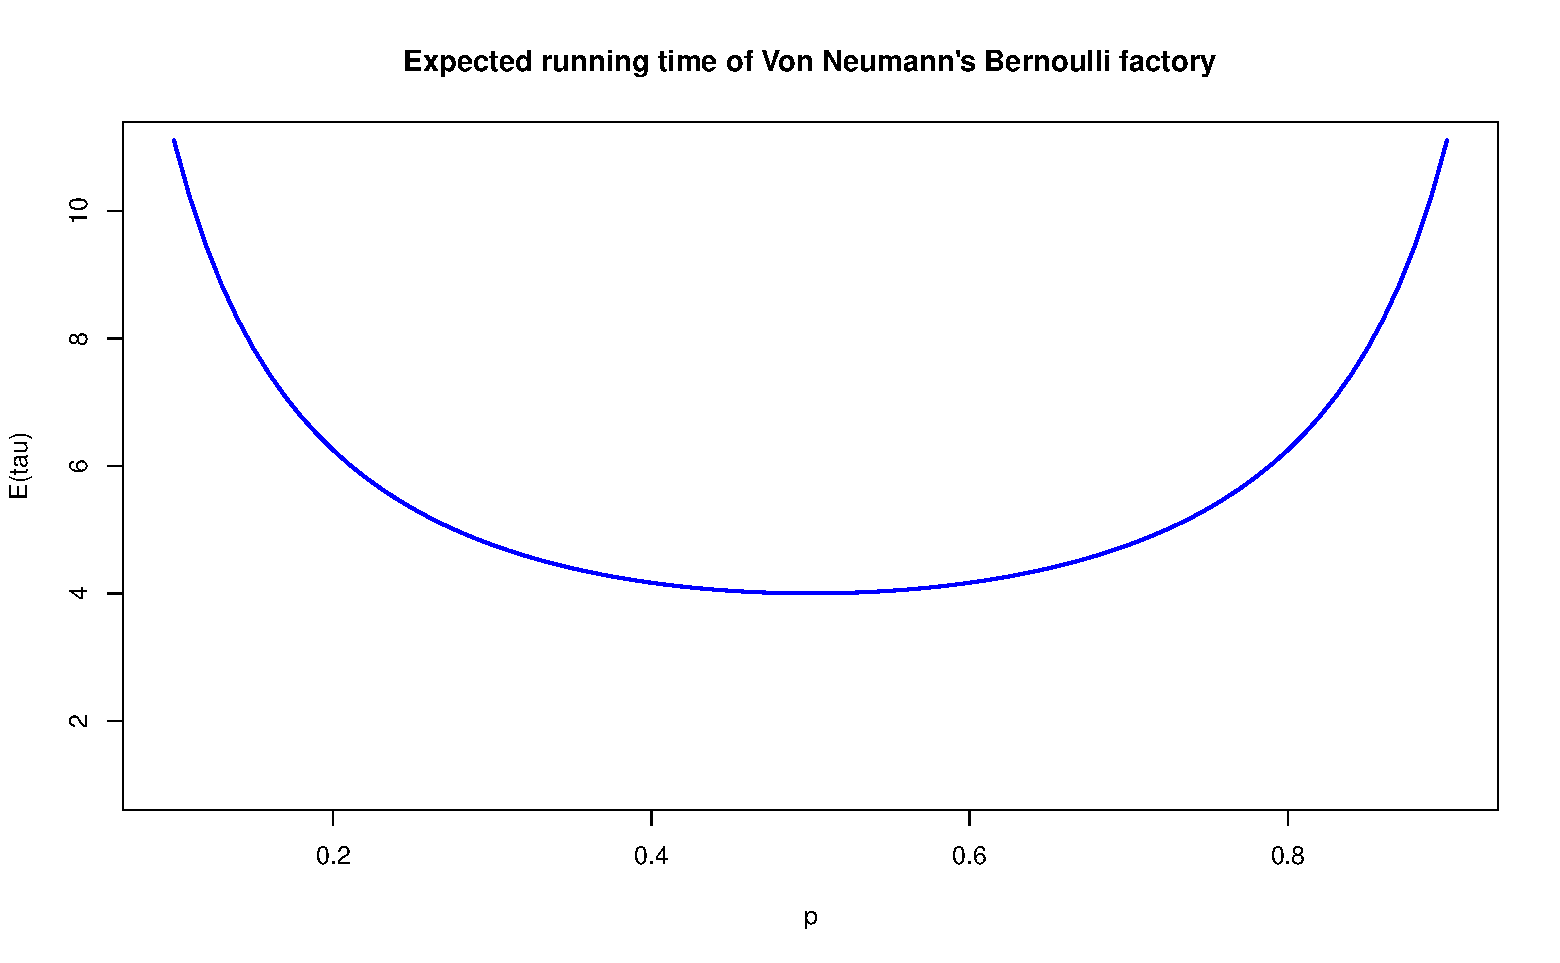
\includegraphics[width=0.8\textwidth]{vonneumann_runtime.pdf}
\caption{•}\label{fig:vonneumann_runtime}
\end{figure}
\end{example}

\begin{example}
$f(p) = p^k, k\in\{1,2,\dots\}$.\\
This problem is solved easily by flipping the coin $k$ times and outputting heads only if all $k$ flips return heads. Again no auxiliary random variable is required.
\begin{align*}
& \tau = k \\
& \A(X_1,\dots,X_T) = \mathbb{I}\{X_1 =1, X_2=1 ,\dots,X_\tau=1\}
\end{align*}
In this case the running time is deterministically equal to $k$. The procedure can be sped up if we allow a random running time, still bounded above by $k$, by stopping the process early if tails comes up. In this case we have
\begin{equation*}
\tau = k \wedge \min\{t \in \{1,2,\dots\}:X_t=0 \}
\end{equation*}
and $\tau \eqdist \min\{k, \Geom(1-p)\}$.
Figure \ref{fig:p2_runtime} shows the expected running time of this procedure for $k=2$.
\begin{figure}
\centering
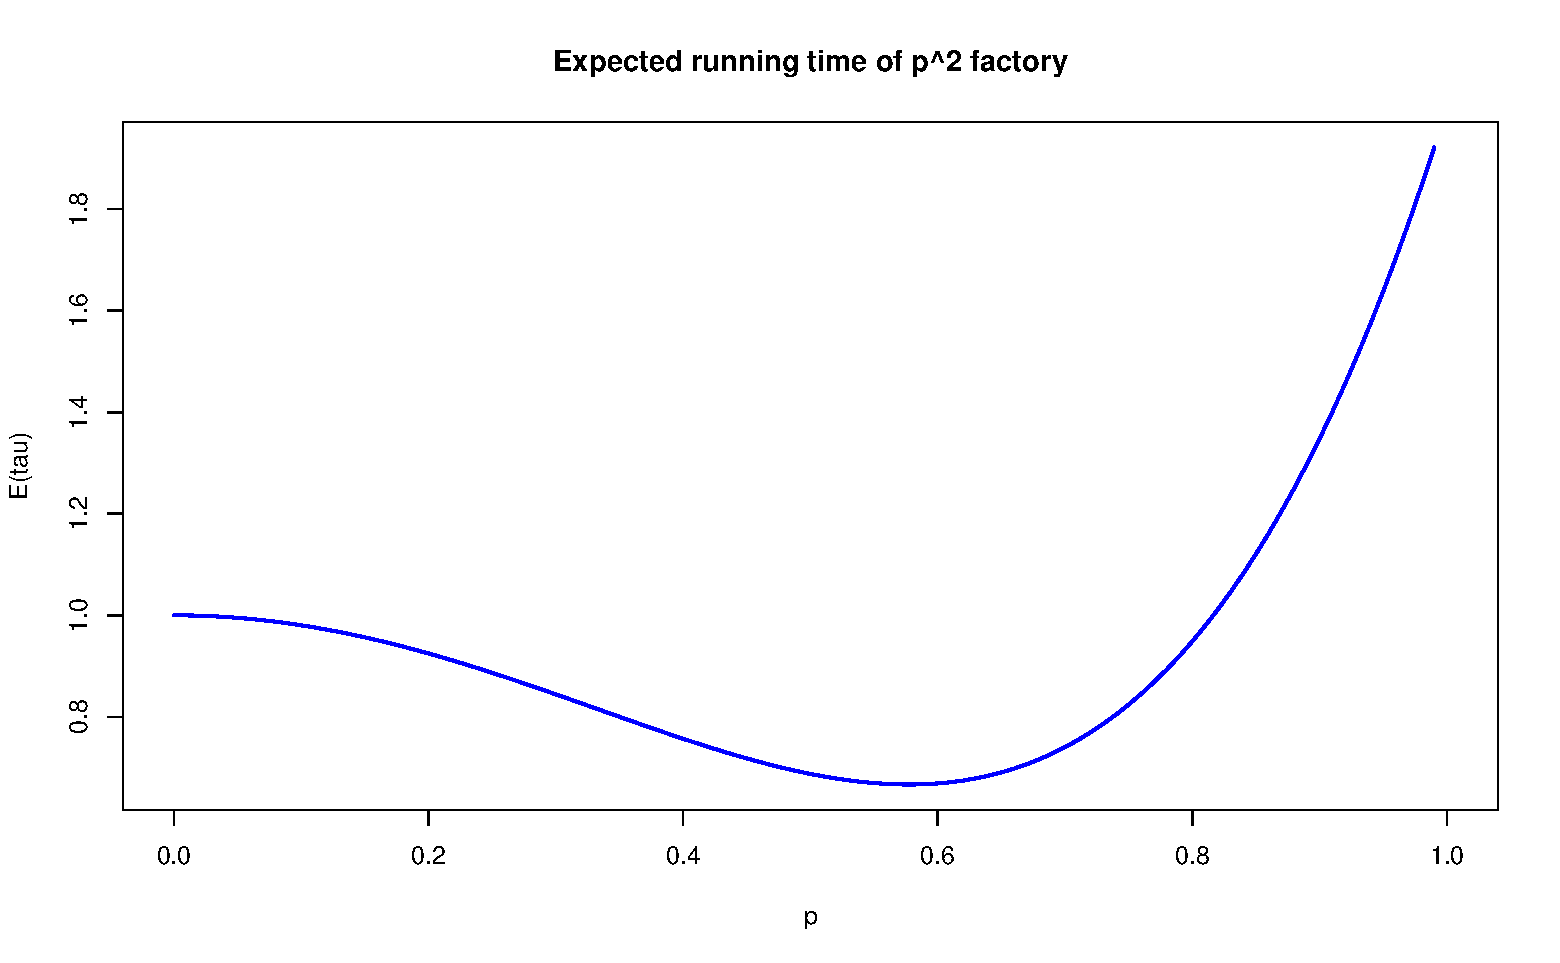
\includegraphics[width=0.8\textwidth]{p2_runtime.pdf}
\caption{•}\label{fig:p2_runtime}
\end{figure}
\end{example}





\bibliography{qbf.bib}
\end{document}